\documentclass[12pt,letterpaper]{article}

\usepackage{fancyhdr,fancybox}
\usepackage{wrapfig}

%% Useful packages
\usepackage{amssymb, amsmath, amsthm} 
%\usepackage{graphicx}  %%this is currently enabled in the default document, so it is commented out here. 
\usepackage{calrsfs}
\usepackage{braket}
\usepackage{mathtools}
\usepackage{lipsum}
\usepackage{tikz}
\usetikzlibrary{cd}
\usepackage{verbatim}
%\usepackage{ntheorem}% for theorem-like environments
\usepackage{mdframed}%can make highlighted boxes of text
%Use case: https://tex.stackexchange.com/questions/46828/how-to-highlight-important-parts-with-a-gray-background
\usepackage{wrapfig}
\usepackage{centernot}
\usepackage{subcaption}%\begin{subfigure}{0.5\textwidth}
\usepackage{pgfplots}
\pgfplotsset{compat=1.13}
\usepackage[colorinlistoftodos]{todonotes}
\usepackage[colorlinks=true, allcolors=blue]{hyperref}
\usepackage{xfrac}					%to make slanted fractions \sfrac{numerator}{denominator}
\usepackage{enumitem}            
    %syntax: \begin{enumerate}[label=(\alph*)]
    %possible arguments: f \alph*, \Alph*, \arabic*, \roman* and \Roman*
\usetikzlibrary{arrows,shapes.geometric,fit}

\DeclareMathAlphabet{\pazocal}{OMS}{zplm}{m}{n}
%% Use \pazocal{letter} to typeset a letter in the other kind 
%%  of math calligraphic font. 

%% This puts the QED block at the end of each proof, the way I like it. 
\renewenvironment{proof}{{\bfseries Proof}}{\qed}
\makeatletter
\renewenvironment{proof}[1][\bfseries \proofname]{\par
  \pushQED{\qed}%
  \normalfont \topsep6\p@\@plus6\p@\relax
  \trivlist
  %\itemindent\normalparindent
  \item[\hskip\labelsep
        \scshape
    #1\@addpunct{}]\ignorespaces
}{%
  \popQED\endtrivlist\@endpefalse
}
\makeatother

%% This adds a \rewnewtheorem command, which enables me to override the settings for theorems contained in this document.
\makeatletter
\def\renewtheorem#1{%
  \expandafter\let\csname#1\endcsname\relax
  \expandafter\let\csname c@#1\endcsname\relax
  \gdef\renewtheorem@envname{#1}
  \renewtheorem@secpar
}
\def\renewtheorem@secpar{\@ifnextchar[{\renewtheorem@numberedlike}{\renewtheorem@nonumberedlike}}
\def\renewtheorem@numberedlike[#1]#2{\newtheorem{\renewtheorem@envname}[#1]{#2}}
\def\renewtheorem@nonumberedlike#1{  
\def\renewtheorem@caption{#1}
\edef\renewtheorem@nowithin{\noexpand\newtheorem{\renewtheorem@envname}{\renewtheorem@caption}}
\renewtheorem@thirdpar
}
\def\renewtheorem@thirdpar{\@ifnextchar[{\renewtheorem@within}{\renewtheorem@nowithin}}
\def\renewtheorem@within[#1]{\renewtheorem@nowithin[#1]}
\makeatother

%% This makes theorems and definitions with names show up in bold, the way I like it. 
\makeatletter
\def\th@plain{%
  \thm@notefont{}% same as heading font
  \itshape % body font
}
\def\th@definition{%
  \thm@notefont{}% same as heading font
  \normalfont % body font
}
\makeatother

%===============================================
%==============Shortcut Commands================
%===============================================
\newcommand{\ds}{\displaystyle}
\newcommand{\B}{\mathcal{B}}
\newcommand{\C}{\mathbb{C}}
\newcommand{\F}{\mathbb{F}}
\newcommand{\N}{\mathbb{N}}
\newcommand{\R}{\mathbb{R}}
\newcommand{\Q}{\mathbb{Q}}
\newcommand{\T}{\mathcal{T}}
\newcommand{\Z}{\mathbb{Z}}
\renewcommand\qedsymbol{$\blacksquare$}
\newcommand{\qedwhite}{\hfill\ensuremath{\square}}
\newcommand*\conj[1]{\overline{#1}}
\newcommand*\closure[1]{\overline{#1}}
\newcommand*\mean[1]{\overline{#1}}
%\newcommand{\inner}[1]{\left< #1 \right>}
\newcommand{\inner}[2]{\left< #1, #2 \right>}
\newcommand{\powerset}[1]{\pazocal{P}(#1)}
%% Use \pazocal{letter} to typeset a letter in the other kind 
%%  of math calligraphic font. 
\newcommand{\cardinality}[1]{\left| #1 \right|}
\newcommand{\domain}[1]{\mathcal{D}(#1)}
\newcommand{\image}{\text{Im}}
\newcommand{\inv}[1]{#1^{-1}}
\newcommand{\preimage}[2]{#1^{-1}\left(#2\right)}
\newcommand{\script}[1]{\mathcal{#1}}


\newenvironment{highlight}{\begin{mdframed}[backgroundcolor=gray!20]}{\end{mdframed}}

\DeclarePairedDelimiter\ceil{\lceil}{\rceil}
\DeclarePairedDelimiter\floor{\lfloor}{\rfloor}

%===============================================
%===============My Tikz Commands================
%===============================================
\newcommand{\drawsquiggle}[1]{\draw[shift={(#1,0)}] (.005,.05) -- (-.005,.02) -- (.005,-.02) -- (-.005,-.05);}
\newcommand{\drawpoint}[2]{\draw[*-*] (#1,0.01) node[below, shift={(0,-.2)}] {#2};}
\newcommand{\drawopoint}[2]{\draw[o-o] (#1,0.01) node[below, shift={(0,-.2)}] {#2};}
\newcommand{\drawlpoint}[2]{\draw (#1,0.02) -- (#1,-0.02) node[below] {#2};}
\newcommand{\drawlbrack}[2]{\draw (#1+.01,0.02) --(#1,0.02) -- (#1,-0.02) -- (#1+.01,-0.02) node[below, shift={(-.01,0)}] {#2};}
\newcommand{\drawrbrack}[2]{\draw (#1-.01,0.02) --(#1,0.02) -- (#1,-0.02) -- (#1-.01,-0.02) node[below, shift={(+.01,0)}] {#2};}

%***********************************************
%**************Start of Document****************
%***********************************************
 %find me at /home/trevor/texmf/tex/latex/tskpreamble_nothms.tex
%===============================================
%===============Theorem Styles==================
%===============================================

%================Default Style==================
\theoremstyle{plain}% is the default. it sets the text in italic and adds extra space above and below the \newtheorems listed below it in the input. it is recommended for theorems, corollaries, lemmas, propositions, conjectures, criteria, and (possibly; depends on the subject area) algorithms.
\newtheorem{theorem}{Theorem}
\numberwithin{theorem}{section} %This sets the numbering system for theorems to number them down to the {argument} level. I have it set to number down to the {section} level right now.
\newtheorem*{theorem*}{Theorem} %Theorem with no numbering
\newtheorem{corollary}[theorem]{Corollary}
\newtheorem*{corollary*}{Corollary}
\newtheorem{conjecture}[theorem]{Conjecture}
\newtheorem{lemma}[theorem]{Lemma}
\newtheorem*{lemma*}{Lemma}
\newtheorem{proposition}[theorem]{Proposition}
\newtheorem*{proposition*}{Proposition}
\newtheorem{problemstatement}[theorem]{Problem Statement}


%==============Definition Style=================
\theoremstyle{definition}% adds extra space above and below, but sets the text in roman. it is recommended for definitions, conditions, problems, and examples; i've alse seen it used for exercises.
\newtheorem{definition}[theorem]{Definition}
\newtheorem*{definition*}{Definition}
\newtheorem{condition}[theorem]{Condition}
\newtheorem{problem}[theorem]{Problem}
\newtheorem{example}[theorem]{Example}
\newtheorem*{example*}{Example}
\newtheorem*{counterexample*}{Counterexample}
\newtheorem*{romantheorem*}{Theorem} %Theorem with no numbering
\newtheorem{exercise}{Exercise}
\numberwithin{exercise}{section}
\newtheorem{algorithm}[theorem]{Algorithm}

%================Remark Style===================
\theoremstyle{remark}% is set in roman, with no additional space above or below. it is recommended for remarks, notes, notation, claims, summaries, acknowledgments, cases, and conclusions.
\newtheorem{remark}[theorem]{Remark}
\newtheorem*{remark*}{Remark}
\newtheorem{notation}[theorem]{Notation}
\newtheorem*{notation*}{Notation}
%\newtheorem{claim}[theorem]{Claim}  %%use this if you ever want claims to be numbered
\newtheorem*{claim}{Claim}


%%
%% Page set-up:
%%
\pagestyle{empty}
\lhead{\textsc{221 - Topology} \\ } %=================UPDATE THIS=================%
\rhead{\textsc{McAmmond, Winter 2019} \\ Trevor Klar}
%\chead{\Large\textbf{A New Integration Technique \\ }}
\renewcommand{\headrulewidth}{0pt}
%
\renewcommand{\footrulewidth}{0pt}
%\lfoot{
%Office: \quad \quad \, M 2-3 \, \, SH 6431x \\
%Math Lab: \, W 12-2 \, SH 1607
%}
%\rfoot{trevorklar@math.ucsb.edu}


\setlength{\parindent}{0in}
\setlength{\textwidth}{7in}
\setlength{\evensidemargin}{-0.25in}
\setlength{\oddsidemargin}{-0.25in}
\setlength{\parskip}{.5\baselineskip}
\setlength{\topmargin}{-0.5in}
\setlength{\textheight}{9in}

\setlist[enumerate,1]{label=\textbf{\arabic*.}}

\begin{document}
\pagestyle{fancy}
\begin{center}
{\Large Homework 1}%=================UPDATE THIS=================%
\end{center}

\begin{enumerate}
\item Construct an explicit deformation retraction of the torus with one point deleted
onto a graph consisting of two circles intersecting in a point, namely, longitude and
meridian circles of the torus.

\answer
Let $T$ be the torus given by $\quotient{\R^2}{\Z^2}$ with one point $\hat p=(\hat{x},\hat{y})$ removed, and let two longitude and meridian circles be the lines $y=b$ and $x=a$, respectively. Denote the union of these two circles $C$.
\jpg{width=0.66\textwidth}{hw1-p1}
We can choose our coordinate system however we like, so \Wlog{} suppose $a=b=0$. Then let $F:T\times [0,1]\to T$ be given by 
$$F(p,t)=\big(1-t\big)p+t\big(\hat{p}+\lambda(p-\hat p)\big),$$
where $\lambda$ is the scalar such that $F(p,1)$ lies on C:%the "square" formed by the two intersecting circles:
\jpg{width=0.20\textwidth}{hw1-p1-2}
We can find $\lambda$ explicitly as a function of $p=(x,y)$ by constraining $\lambda$ to be the minimum positive defined quantity from the following list: $\left(\frac{1-\hat x}{x-\hat x}, \frac{1-\hat y}{y-\hat y},\frac{-\hat x}{x-\hat x}, \frac{-\hat y}{y-\hat y}\right)$. 

Then 
\begin{itemize}
\item $F(p,0)=p$, 
\item $F(p,1)\in C$ for all $p\in T$, 
\item for all $p\in C$ one can check that $\lambda=1$, so $F(p,t)=p$ for all time $t$,
\item $F$ is continuous. 
\end{itemize}
This last point is perhaps not trivial, since we must show that $\lambda$ is a continuous function of $p$. To see this, partition the torus into 4 regions by connecting the corners to $\hat p$: 
\jpg{width=0.20\textwidth}{hw1-p1-3}
Each region has a corresponding $\lambda$-value from the above list, and they agree on their boundaries (that is, for any $p$ on a boundary line, the expressions on each side of the line give the same values for $\lambda$). In the interior of each region, $\lambda$ is determined by its equation for that region, which is continuous. Thus $\lambda(p)$ is continuous, and so is $F$. 
\qed

\item Construct an explicit deformation retraction of $\R^n - \{0\}$ onto $S^{n-1}$. 

\answer Let $F(p,t)=p(1-t)+\frac{p}{\norm{p}}(t)$. Then 
\begin{itemize}
\item $F(p,0)=p$, 
\item $F(p,1)\in S^{n-1}$ for all $p\in T$, since $\frac{p}{\norm{p}}$ has norm $1$, 
\item for all $p\in S^{n-1}$, we have that $F(p,t)=p(1-t)+p(t)=p$, so $F$ fixes every point in $S^{n-1}$,
\item $F$ is continuous since $p\neq0$ so the denominator in $F$ never vanishes.
\end{itemize}\qed

\pagebreak
\item 
\begin{enumerate}[label=(\alph*)]
\item Show that the composition of homotopy equivalences $X\to Y$ and $Y\to Z$ is a
homotopy equivalence $X\to Z$. Deduce that homotopy equivalence is an equivalence
relation.
\begin{proof}
By assumption, there exist homotopy equivalence maps $f,\bar{f}, g, \bar{g}$ such that ${\bar{f}f\simeq\id_X}$ and ${\bar{g}g\simeq\id_Y}$. This means that $gf:X\to Z$ is a homotopy equivalence map, since 
$$gf\bar{f}\bar{g}\simeq g\id_Y \bar{g} = g\bar{g} \simeq \id_Z$$ 
and
$$\bar{f}\bar{g}gf\simeq f\id_Y \bar{f} = f\bar{f} \simeq \id_X. $$
thus 
\begin{itemize}
\item $X \simeq X$, since $\id_X$ is a homotopy equivalence map,
\item $X \simeq Y \implies Y \simeq X$ by definition of a homotopy equivalence map, and 
\item $X\simeq Y$ and $Y\simeq Z \implies X \simeq Z$ as shown above. \qedwhite 
\end{itemize}
\let\qed\relax
\end{proof}

\item Show that the relation of homotopy among maps $X\to Y$ is an equivalence relation.
\begin{proof} Let $f,g,h:X\to Y$ be maps. 
\begin{itemize}
\item $f \simeq f$ since $F(x,t) = f(x) \; \forall t$ is a homotopy. 
\item If $f\simeq g$ with $F(x,0)=f(x)$ and $F(x,1)=g(x)$, then $F(x,(1-t))$ is a homotopy so $g \simeq f$. 
\item If $\phi_1$ is a homotopy relating $f$ and $g$ and $\phi_2$ is a homotopy relating $g$ and $h$, then 
$$F(x,t)=
\begin{cases}
\phi_1(x,2t) & t\in[0,\frac{1}{2}] \\ 
\phi_2(x,2(t-\frac{1}{2})) & t\in(\frac{1}{2}, 1]
\end{cases}
$$
is a homotopy relating $f$ and $h$.\qedwhite
\end{itemize}
\let\qed\relax
\end{proof}

\item Show that a map homotopic to a homotopy equivalence is a homotopy equivalence. 
\begin{proof}
Let $f,g,\bar{g}:X\to Y$ such that $g\circ\bar{g}\simeq\id$ and $f\simeq g$ with $\begin{array}{ll}
F(x,0)=f(x)\\
F(x,1)=g(x)
\end{array}$. 

Then considering the map $F(\bar{g}(x),t)$\footnote{We know that compositions and restrictions of maps are maps, so we won't get bogged down in mentioning that detail in this or further proofs.}, we find that 
$\begin{array}{ll}
F(\bar{g}(x),0)=f\circ \bar{g}(x)\\
F(\bar{g}(x),1)=g \circ \bar{g}(x)
\end{array}$
so $f\bar{g}\simeq g\bar{g} \simeq \id$, and similarly 
$\begin{array}{ll}
\bar{g}(F(x,0))=\bar{g}\circ f(x)\\
\bar{g}(F(x,1))=\bar{g} \circ g(x)
\end{array}$ so $\bar{g}f\simeq \bar{g}g \simeq \id$. 
\end{proof}
\end{enumerate}

\vfill
\pagebreak
\begin{definition*}
A \emph{deformation retraction in the weak sense} of a space $X$ to a subspace $A$ is a homotopy $f_t: X\to X$ such that $f_0 = \id$, $f_1(X) \subset A$, and $f_t(A) \subset A$ for all $t$. 
\end{definition*}

\item Show that if $X$ deformation retracts to $A$ in the weak sense, then the inclusion $\iota:A ֓\hookrightarrow X$ is a homotopy equivalence.
\begin{proof}
Denote $f_1(x)$ by $g(x)$, a map $X\to A$. Then $\iota \circ g = g\simeq \id_X$ by assumption, and since $g\circ\iota=g|_A$ and $f_t|_A$ is a homotopy between $g|_A$ and $\id_X|_A=\id_A$, then $g\circ\iota=g|_A\simeq\id_A$. 
\end{proof}


\item Show that if a space $X$ deformation retracts to a point $x \in X$ , then for each neighborhood $U$ of $x$ in $X$ there exists a neighborhood $V \subset U$ of $x$ such that the inclusion map $V\hookrightarrow U$ is nullhomotopic.

\begin{proof}\mbox{}

%\begin{minipage}{0.60\linewidth}
Let $F:X\times I \to X$ be the above deformation retraction. We want to produce an open set of points which are in $U$, and which remain in $U$ for all time $t$. 
%\end{minipage}

\begin{minipage}{\linewidth}
\begin{center}
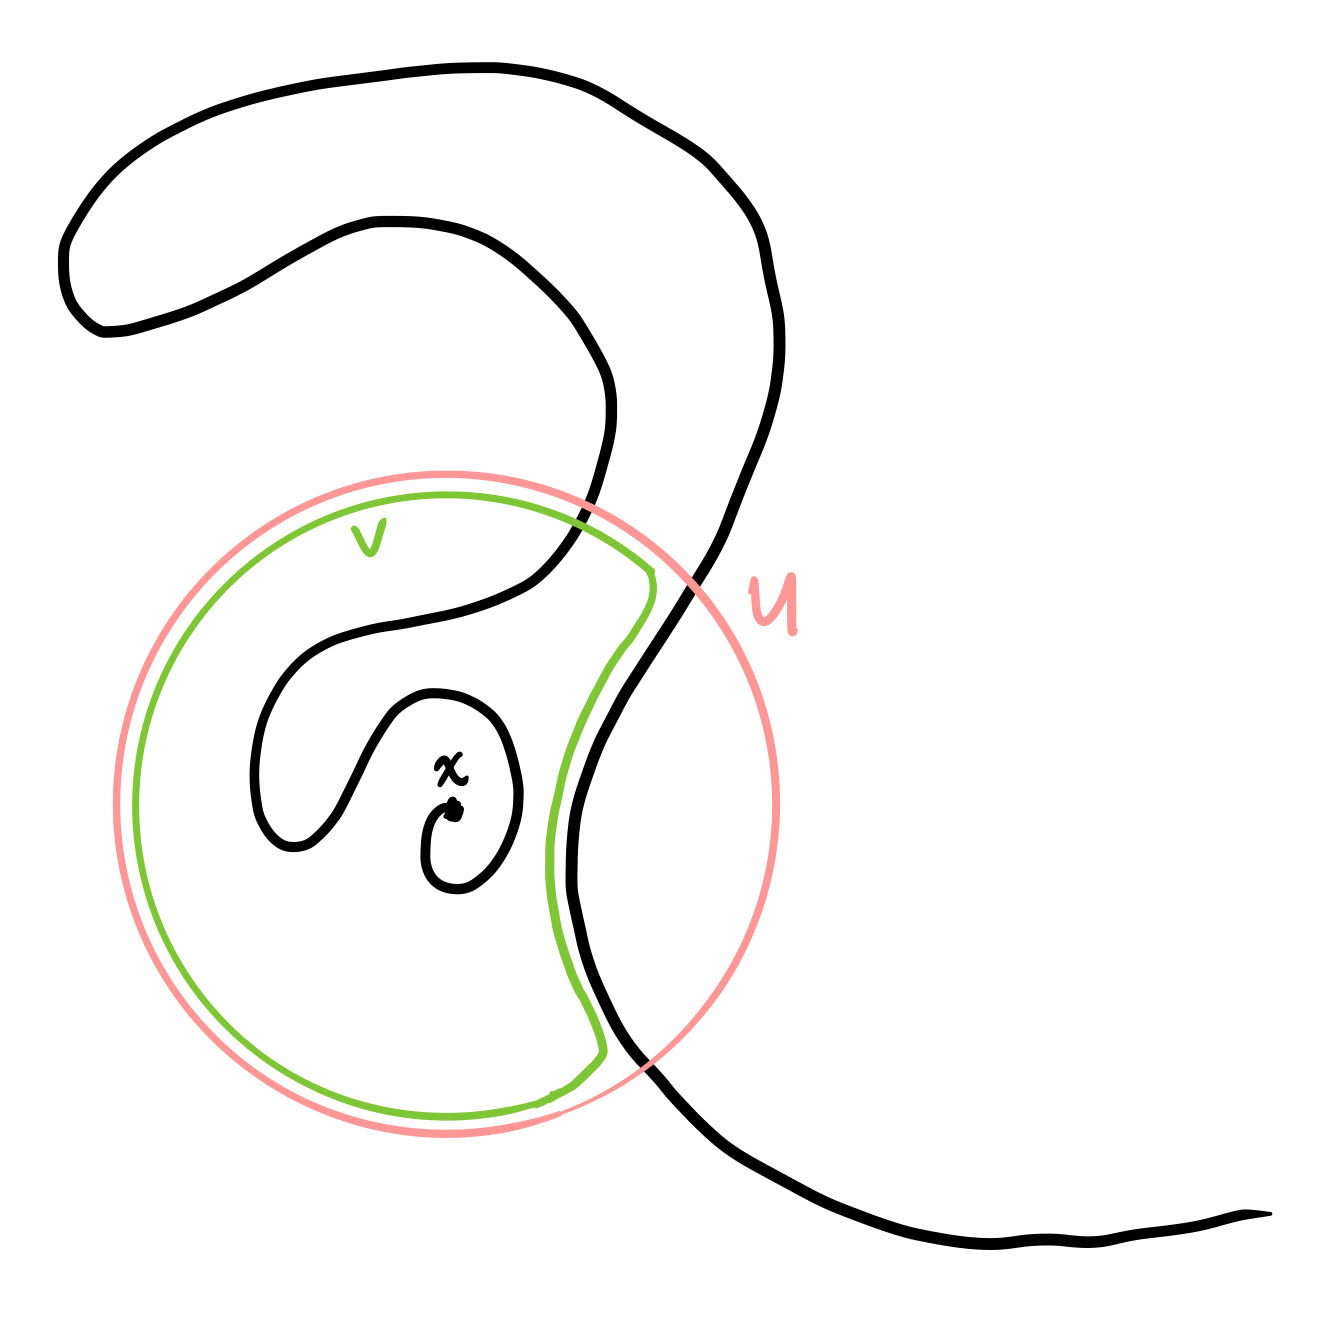
\includegraphics[height=1.2in]{hw1-p5-1}
\end{center}
\vspace{-4ex}
\captionof*{figure}{\footnotesize We should exclude the points in $U$ which leave $U$ as $t\to 1$.}
\end{minipage}

Thus we take $(U\times I) \cap \preimage{F}{U}$, which gives us the set of all $(x,t)$ such that the point begins in $U$, and is in $U$ at some time $t$. 

\begin{minipage}{\linewidth}
\begin{center}
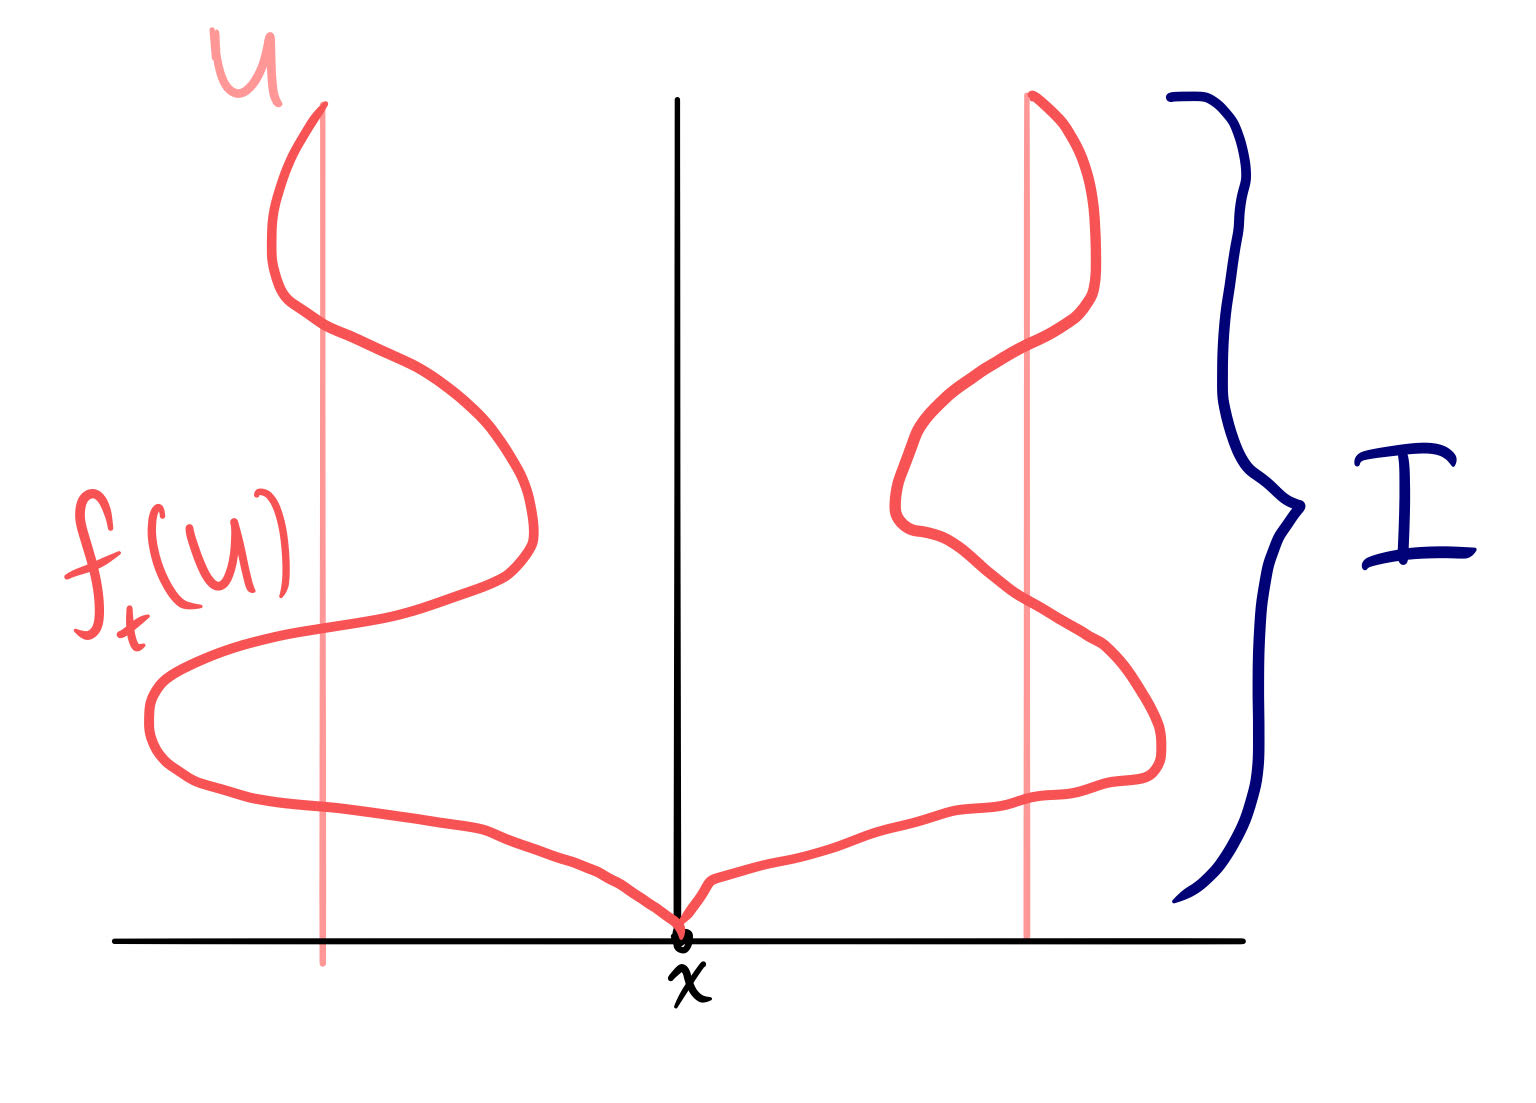
\includegraphics[height=1.2in]{hw1-p5-2}
\end{center}
\vspace{-4ex}
%\captionof*{figure}{\footnotesize We should exclude the points in $U$ which leave $U$ as $t$ varies.}
\end{minipage}

Now $(U\times I) \cap \preimage{F}{U}$ is open in the product topology on $X\times I$, so for every point $(x,t) \in \{x\}\times I$, we choose an open rectangle $V_t\subset \{x\}\times I$ containing $(x,t)$, and observe that $\{V_t\}_{t\in I}$ is an open cover of $\{x\}\times I$, a compact space. Thus we can obtain a finite subcover $\{V_i\}$. 

\begin{minipage}{\linewidth}
\begin{center}
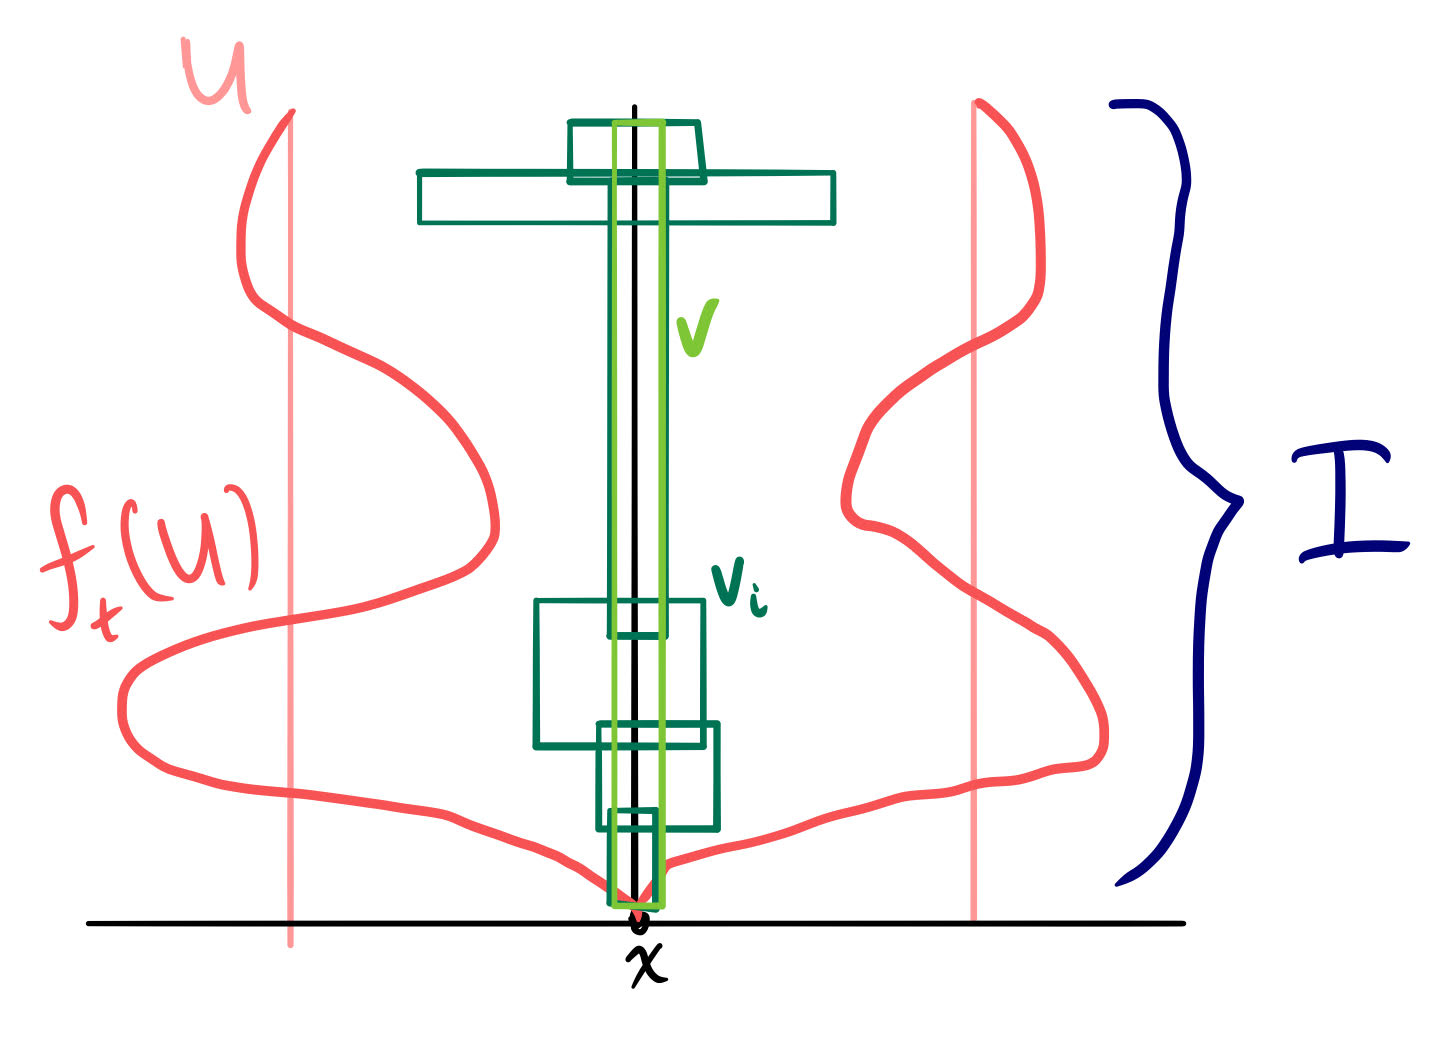
\includegraphics[height=1.2in]{hw1-p5-3}
\end{center}
\vspace{-4ex}
\captionof*{figure}{\footnotesize (In this figure $V$ should be labeled $V\times I$, and $U$ should be $U\times I$.)}
\end{minipage}

Let $V=\bigcap_i\proj{X}{V_i}$. Then for any $p \in V$, $(p,t)\in \bigcup_i V_i \subset (U\times I) \cap \preimage{F}{U}$ for all $t$, so that point remains in $V$ for all time. To finish the proof, observe that $F|_V$ is a homotopy between the inclusion map $V\hookrightarrow U$ and the constant map $x$. 
\end{proof}


\pagebreak
\item 
	\begin{enumerate}[label=(\alph*)]
	\item \mbox{}\\ 
	\begin{minipage}{.8\linewidth}
	\vspace{-4ex}Let $X$ be the subspace of $\R^2$ consisting of the horizontal segment $[0, 1]\times \{0\}$ together with all the vertical segments $\{r \}\times[0, 1 - r ]$ for
$r$ a rational number in $[0, 1]$. Show that $X$ deformation retracts to
any point in the segment $[0, 1]\times \{0\}$, but not to any other point. [See
the preceding problem.]
	\end{minipage}
	\begin{minipage}{.2\linewidth}
	\vspace{-4ex}	
	\begin{center}
	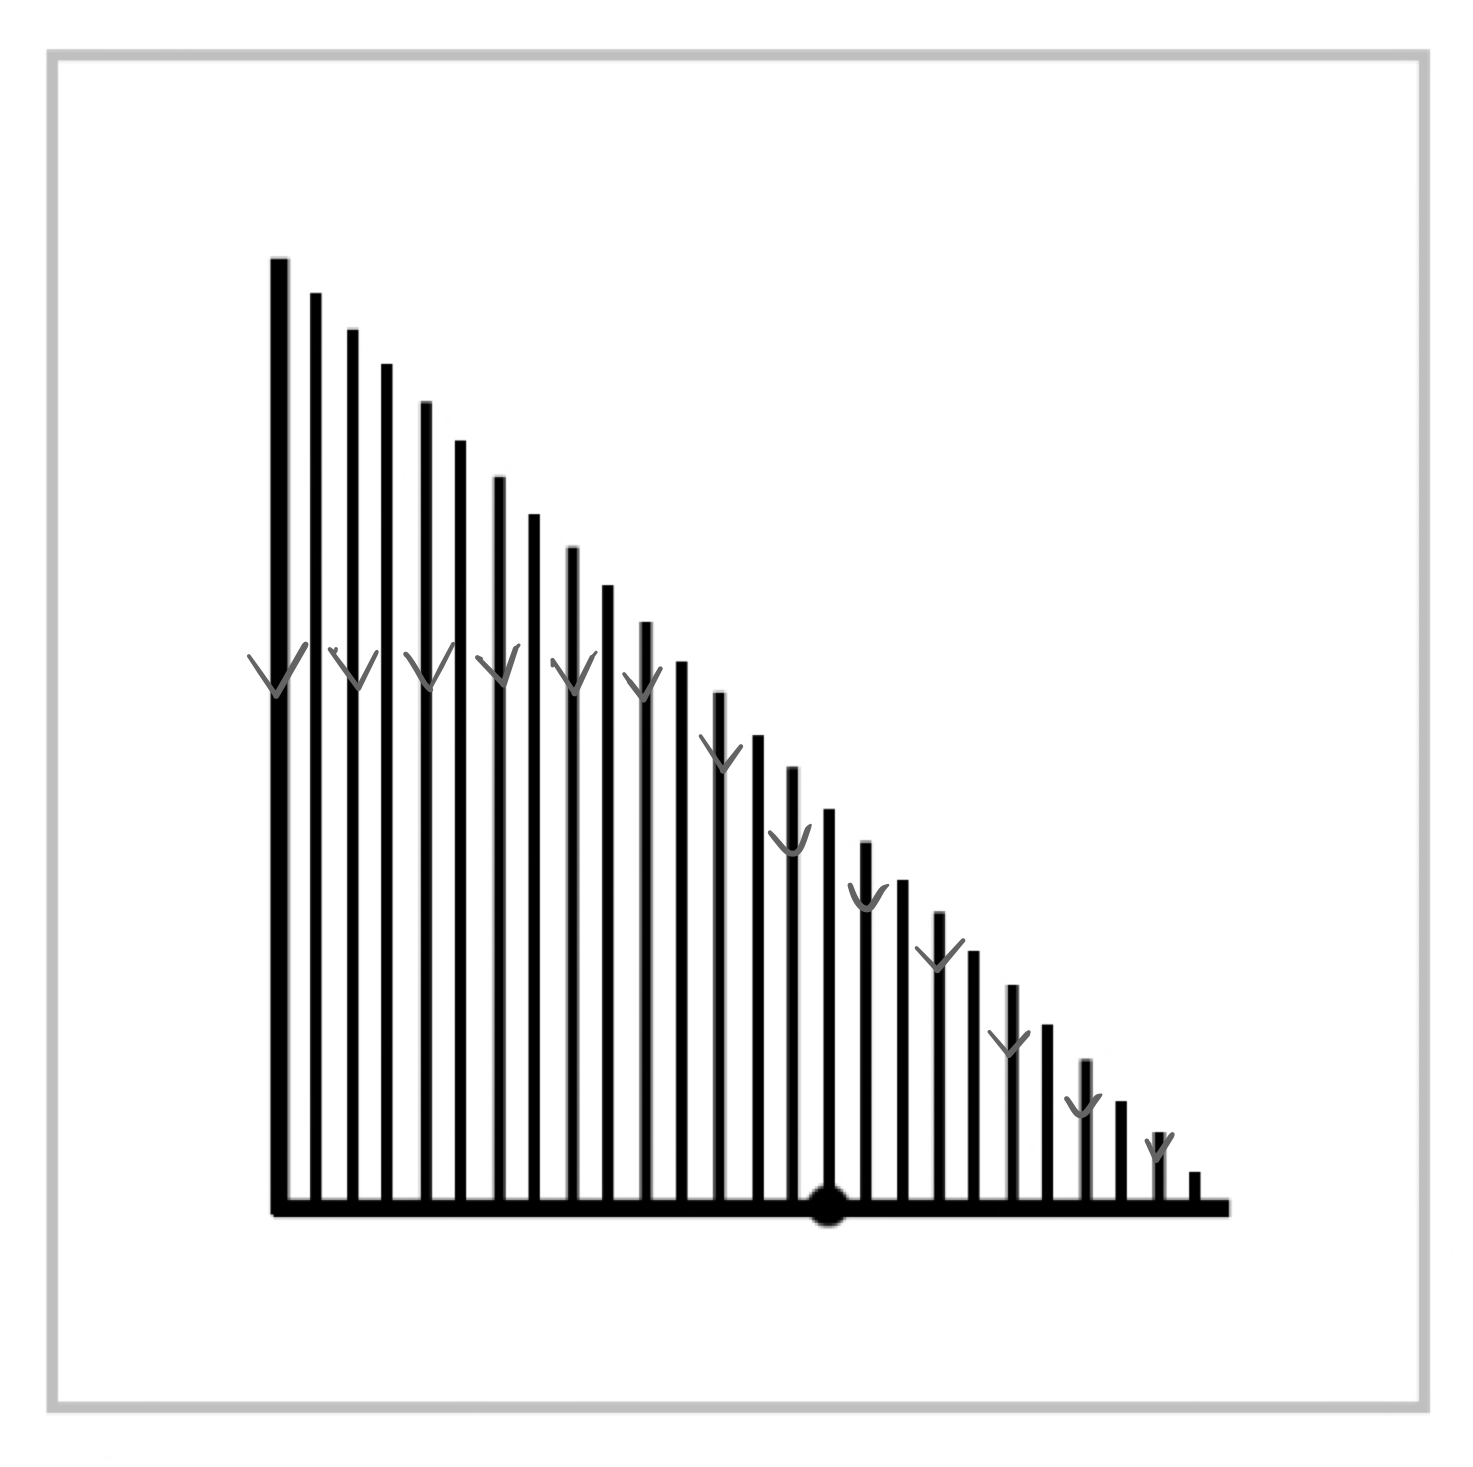
\includegraphics[height=1.2in]{hw1-p6-1}
	\end{center}
	\end{minipage}
	
	\begin{proof}
	We can deformation retract all the tines down to $x$-axis, then retract in to the desired point, as shown in the figures:
	\begin{center}	
	\raisebox{-.45\height}{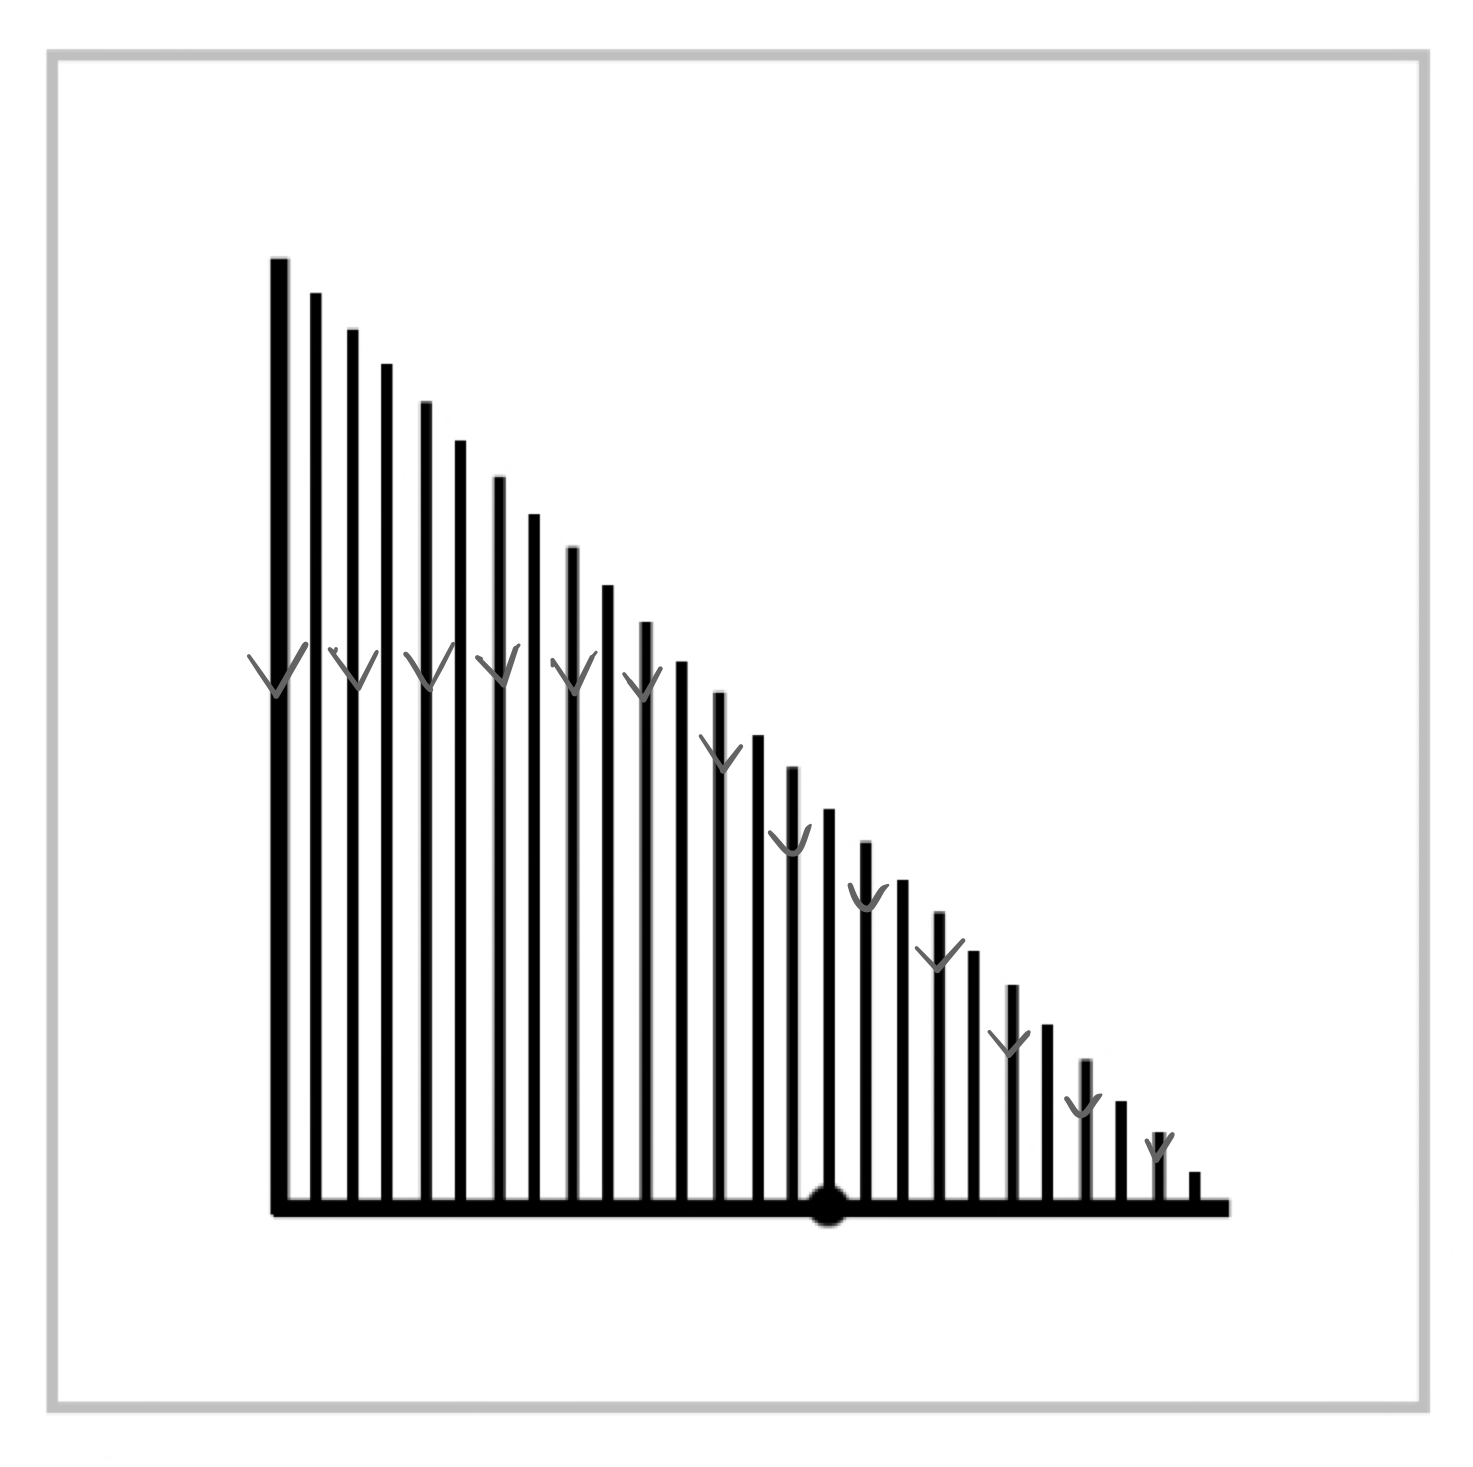
\includegraphics[height=1.2in]{hw1-p6-1}}
  $\simeq$
	\raisebox{-.45\height}{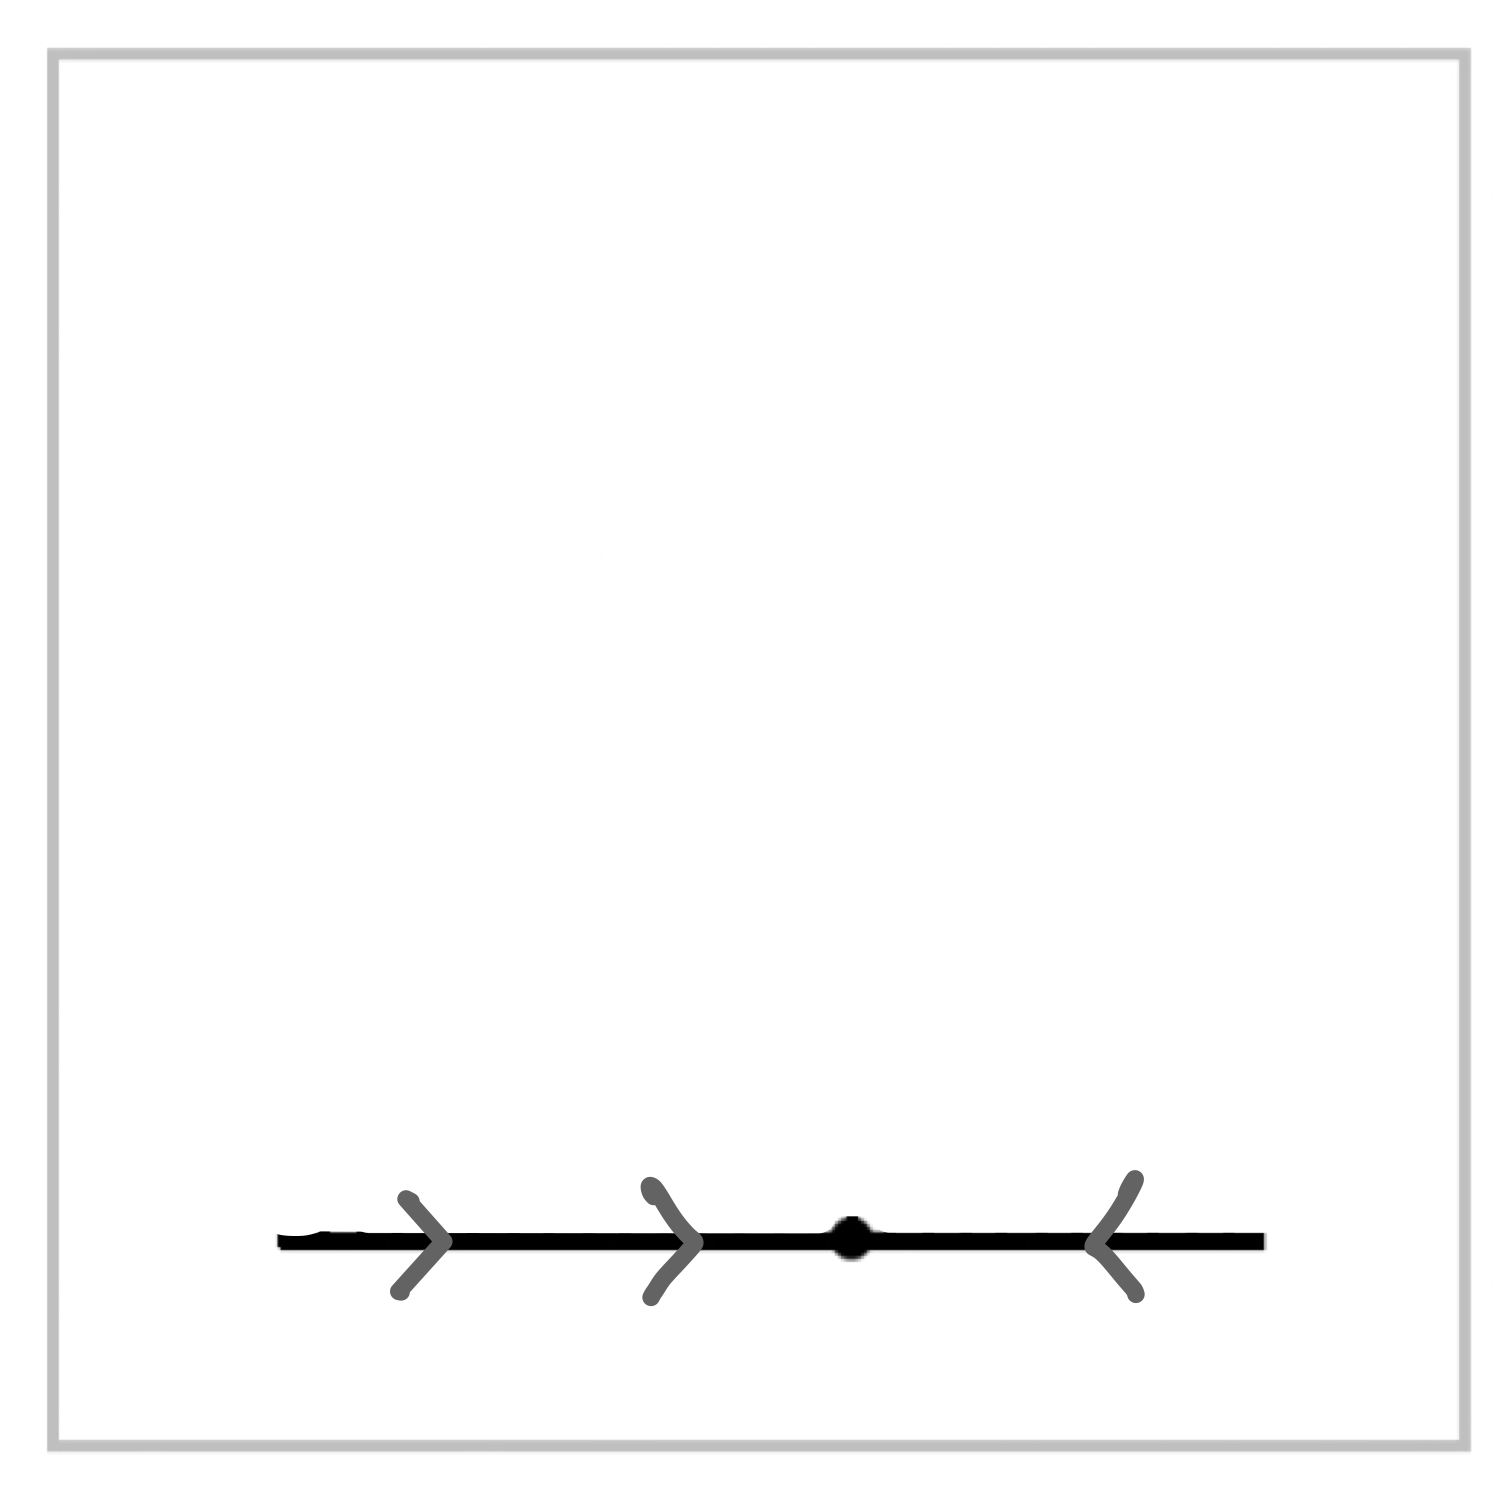
\includegraphics[height=1.2in]{hw1-p6-2}}
  $\simeq$
	\raisebox{-.45\height}{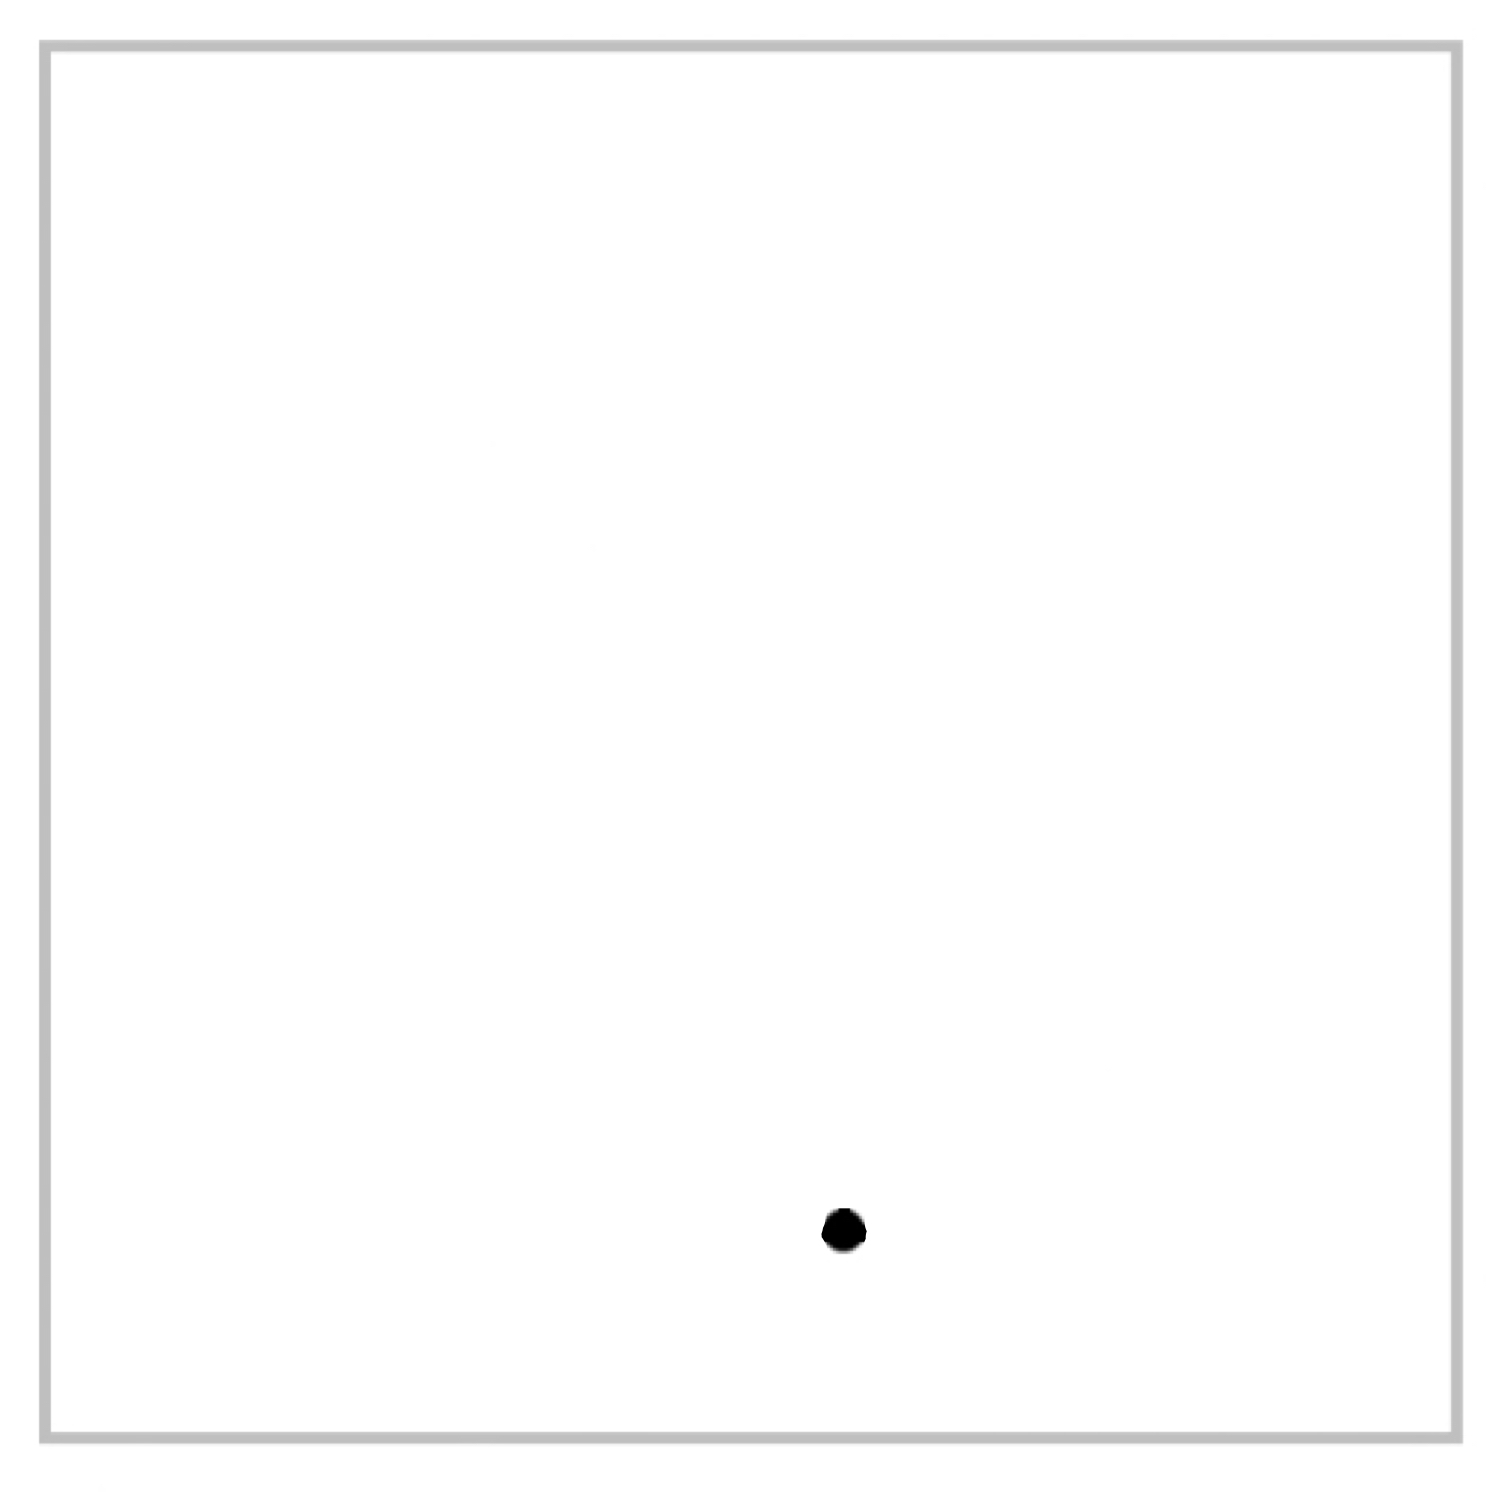
\includegraphics[height=1.2in]{hw1-p6-3}}
	\end{center}
	This fails however if we try to retract to a point on one of the tines, because there are other tines arbitrarily close to the one in question, and they cannot be retracted continuously. In general, no deformation retraction to a point on the tines can exist, because every neighborhood of such a point contains disconnected pieces of other tines, and the identity map on such a neighborhood cannot be nullhomotopic. 	
	\end{proof}		
	
	\item Let $Y$ be the subspace of $\R^2$ that is the union of an infinite number of copies of $X$ arranged as in the figure below. Show that $Y$ is contractible but does not deformation retract onto any point.
	\jpg{width=\linewidth}{hw1-p6-4}		
	\item Let $Z$ be the zigzag subspace of $Y$ homeomorphic to $\R$ indicated by the heavier
line. Show there is a deformation retraction in the weak sense (see Exercise 4) of $Y$ onto $Z$ , but no true deformation retraction.
	\begin{proof}
	To see that $Y$ does not deformation retract onto any point (b), note that it cannot retract to a point on the tines for the same reason as in part (a), and every segment of $Y$ is a tine for some part of the figure. 
	
	\pagebreak
	To see that $Y$ is contractible (b), we will produce a deformation retraction in the weak sense of $Y$ onto $Z$ (c), and then observe that $Z$ is homeomorphic to $\R$ which is homotopy equivalent to a point. 
	
	Each point has an obvious way to move continuously along $Y$ in a rightwards direction; moving down the tines until it is on $Z$, and then zig-zagging on $Z$ forever. 
	\jpg{width=0.8\linewidth}{hw1-p6-6}	
	Moving all the points at a constant speed keeps all points moving rightwards together, so that only their vertical spacing changes: 
	
	\jpg{width=0.8\linewidth}{hw1-p6-5}	
	
	and after moving for 1 second, every point lies on $Z$. Thus the homotopy described above is such that $F(x,0)=x$, $F(x,1)\in Z$, and $f(z,t)\in Z$ for all $z\in Z$. 
	
	To complete the proof, we can choose any point $p$ in $X$ and contract $Z$ in the same way we would $\R$, all in to the point $p$. The composition of these two homotopies gives a homotopy between $\id_Y$ and the constant map $p$. 
	\end{proof}
	
	\end{enumerate}

\end{enumerate}

\vfill

Collaborators:
\begin{enumerate}
\item Zach Wagner, Nick Bragman, Kyle Hansen

\item

\item

\item

\item Leslie Mavrakis

\item Zach Wagner, Christian Hong (not in this class, but helped me find a key mistake). 
\end{enumerate}
\end{document}



